\documentclass[lettersize,journal]{IEEEtran}

\usepackage{amsmath,amsfonts,amssymb}
\usepackage{array}
\usepackage{textcomp}
\usepackage{stfloats}
\usepackage{url}
\usepackage{graphicx}
\usepackage{cite}
\usepackage{xcolor}
\usepackage{balance}
\usepackage{booktabs}
\usepackage{tabularx}
\usepackage{ragged2e}
\usepackage{tikz}
\usetikzlibrary{positioning,arrows.meta,calc}

\newcolumntype{Y}{>{\RaggedRight\arraybackslash}X}
\newcolumntype{P}[1]{>{\RaggedRight\arraybackslash}p{#1}}

\begin{document}
	\title{Vision-Based Misalignment Diagnosis of the SOFIA Hexagonal Units: Geometric and Learned Estimators}

	\author{
		Marco Heimdal Castro Magaña, Alejandro Amador Franco, Karen Alejandra Guevara Vasquez, María Alicia Vela Contreras, Juan Pablo Contreras Quiñones,
		Jorge A. Lizarraga, Luis E. González-Jiménez, Luis F. Luque-Vega

		\thanks{The authors are affiliated with the Instituto Tecnológico de Estudios Superiores de Occidente (ITESO), Tlaquepaque, Jalisco, Mexico.}
	}

	\markboth{Laboratory for the Development of Technological Solutions}
	{Vision-Based Misalignment Diagnosis of the SOFIA Units}

	\maketitle

	\begin{abstract}
		Each SOFIA module carries 16 hexagonal plates, each tilted by two servomotors \cite{sofia_architecture}. A plate that does not return to its zero position after a motion is difficult to notice by eye, so this work estimates the two joint angles of every plate from a single overhead photograph and classifies each plate as OK ($<2^\circ$), REVIEW ($2$--$5^\circ$), or MISALIGNED ($>5^\circ$). Four ArUco markers placed at the height of the plates rectify the photograph, and a training-free geometric method, a small convolutional neural network (CNN), and a hybrid rule that combines both are compared on 10\,000 images rendered in Webots with the simulation model of the SOFIA unit. On 1500 test images (24\,000 plates), the CNN obtains a mean absolute error of $0.20^\circ$, a maximum error of $3.3^\circ$, and a state accuracy of 96.8\,\%, and is the most accurate estimator in every range of misalignment, while the geometric method, limited by the short lever arm of the unit, reaches $0.52^\circ$. The estimators are integrated in a diagnosis application with a dedicated processing thread, which can also be connected to a live Webots simulation to misalign the plates interactively and compare each diagnosis with the angles measured in the simulation.
	\end{abstract}

	\begin{IEEEkeywords}
		Misalignment diagnosis, fiducial markers, homography, convolutional neural networks, Webots, synthetic data, multithreading.
	\end{IEEEkeywords}


	\section{Method}

	\subsection{Setup and Synthetic Dataset}

	The module was reproduced in Webots \cite{webots} with 16 instances of the PROTO of the SOFIA unit, generated from its CAD model through URDF with \texttt{urdf2webots} \cite{urdf2webots}. Each unit has two joints with limits of $\pm30^\circ$ whose axes intersect $L=37$~mm below a hexagonal plate of 60~mm (center to vertex), and the plates lie 59~mm above the floor. The units are arranged in four staggered rows with 140~mm between neighbors of the same row and 116~mm between rows, the smallest spacing at which no two plates collide with all of them at their joint limits, computed from the meshes. A frame with four ArUco markers \cite{aruco} (60~mm, dictionary 4$\times$4) surrounds the array, with their centers on a 0.60~m square at the height of the plates, the smallest square that keeps every marker clear of the region swept by the plates. A generator controller set random joint angles, rendered one photograph, and stored the 32 angles measured by the joint sensors as labels. To mimic a hand-placed camera, each image used a camera height of 1.30--1.40~m, tilts of up to $\pm4^\circ$, a yaw of up to $\pm8^\circ$, an offset of up to $\pm4$~cm, and random lights and floor tone. The misalignment of each plate follows the expected operation of the robot: 10\,\% at zero, 60\,\% between $0$ and $5^\circ$, 20\,\% between 5 and $15^\circ$ (a plate moved by hand or jammed), and 10\,\% from $15^\circ$ to the limit, in a random direction; this yields 35\,\% OK, 36\,\% REVIEW, and 29\,\% MISALIGNED plates. Image~0, with every plate at zero, is the reference. The other 9999 images were split \emph{by image} into 6999 for training, 1500 for validation, and 1500 for testing, so the 16 plates of a photograph never fall in different subsets.

	\subsection{Rectification and Crops}

	The pipeline is shown in Fig.~\ref{fig:pipeline}. Since the markers lie in the plane of the plates, the homography computed from their four centers maps that plane exactly to a top view at 1~px/mm ($860\times860$ px), independently of the camera pose. In the rectified image ($720\times720$~px), every plate at zero falls on a known pixel, and a crop of $200\times200$~mm around it is resized to $128\times128$~px. The same rectified image and crops feed all the estimators.

	\begin{figure}[!t]
		\centering
		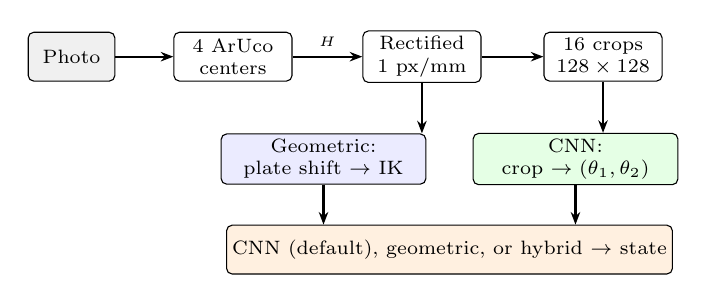
\begin{tikzpicture}[
			font=\scriptsize,
			box/.style={draw, rounded corners=2pt, align=center, minimum height=0.62cm, inner sep=2pt, fill=white},
			arr/.style={-{Stealth[length=1.6mm]}, thick}
			]
			\node[box, fill=gray!12, minimum width=1.1cm] (foto) at (0,0) {Photo};
			\node[box, minimum width=1.5cm] (aruco) at (2.05,0) {4 ArUco\\centers};
			\node[box, minimum width=1.5cm] (rect) at (4.45,0) {Rectified\\1 px/mm};
			\node[box, minimum width=1.5cm] (crop) at (6.75,0) {16 crops\\$128\times128$};
			\node[box, fill=blue!8, minimum width=2.6cm] (geo) at (3.2,-1.3) {Geometric:\\plate shift $\rightarrow$ IK};
			\node[box, fill=green!10, minimum width=2.6cm] (cnn) at (6.4,-1.3) {CNN:\\crop $\rightarrow (\theta_1,\theta_2)$};
			\node[box, fill=orange!12, minimum width=5.6cm] (hib) at (4.8,-2.45) {CNN (default), geometric, or hybrid $\rightarrow$ state};
			\draw[arr] (foto) -- (aruco);
			\draw[arr] (aruco) -- node[above, font=\tiny]{$H$} (rect);
			\draw[arr] (rect) -- (crop);
			\draw[arr] (rect.south) -- (rect.south |- geo.north);
			\draw[arr] (crop.south) -- (crop.south |- cnn.north);
			\draw[arr] (geo.south) -- (geo.south |- hib.north);
			\draw[arr] (cnn.south) -- (cnn.south |- hib.north);
		\end{tikzpicture}
		\caption{Diagnosis pipeline. The homography $H$ maps the plane of the plates to a fixed top view, so every plate appears at a known position.}
		\label{fig:pipeline}
	\end{figure}

	\subsection{Geometric Estimator}

	The plate orientation is $R_x(\theta_1)R_y(\theta_2)(0,0,L)^\top$, so its center moves in the top view by
	\begin{equation}
		\Delta v = L\sin\theta_2, \qquad \Delta u = L\cos\theta_2\sin\theta_1,
	\end{equation}
	which is inverted as $\theta_2=\arcsin(\Delta v/L)$ and $\theta_1=\arcsin\!\big(\Delta u/(L\cos\theta_2)\big)$. In a window around each zero position, the image is binarized with Otsu's method \cite{otsu}, a hexagonal template locates the plate by normalized cross-correlation with sub-pixel refinement, and the centroid of the connected bright region replaces that estimate when its area and solidity match a plate. Displacements are measured with respect to the plates in the reference image, which absorbs small assembly errors. The method needs no training. Its accuracy is limited by the lever arm: with $L=37$~mm, an error of 1~px (1~mm) in the rectified image corresponds to about $1.5^\circ$. In addition, a tilted plate also drops, which perspective converts into a bias at large angles.

	\subsection{Learned Estimators}

	A small CNN maps a crop to $(\theta_1,\theta_2)/30^\circ$ in PyTorch \cite{pytorch}. It is trained from scratch and has five blocks of two $3\times3$ convolutions with batch normalization and max pooling (32--128 channels, 1.28~M parameters). Since the answer is \emph{where} the plate lies in the crop, it omits the global average pooling and flattens the final $4\times4$ feature map into the fully connected head. Training used a smooth-L1 loss, AdamW \cite{adamw} with a one-cycle schedule \cite{onecycle}, mixed precision, and batches of 128, for 25 epochs; the epoch with the lowest validation error was kept. Augmentation applied horizontal and vertical flips, changing the sign of $\theta_1$ or $\theta_2$, respectively, and random gain, gamma, blur, and noise; translations, rotations, and scaling were excluded because they would change the answer. To avoid a bottleneck in the CPU, the 112\,000 training crops are stored in the GPU and each batch is augmented there. In a preliminary experiment with the previous unit model and 2000 images, a ResNet18 \cite{resnet} pretrained on ImageNet (13.3~M parameters) did not outperform the small CNN ($0.29^\circ$ versus $0.25^\circ$ of mean error), so it was not retrained for the final dataset.

	\subsection{Hybrid Rule}

	In the preliminary experiment, the geometric method was the most accurate below $5^\circ$ and the CNN above it, so a per-plate rule was designed to select between them: if the geometric and CNN estimates differ by more than $2^\circ$ on either axis, the CNN value is used and the plate is flagged for inspection; otherwise, the geometric value is used when the CNN places the plate within $6^\circ$ of zero, and the CNN value elsewhere.


	\section{Results}
	\label{sec:results}

	Table~\ref{tab:results} reports the test results on a desktop PC with an AMD Ryzen CPU and an NVIDIA RTX~3060 GPU. The time per photograph includes the marker detection, the rectification, and the estimation of the 16 plates.

	\begin{table}[!t]
		\centering
		\caption{Test Results (1500 Images, 24\,000 Plates)}
		\label{tab:results}
		\scriptsize
		\setlength{\tabcolsep}{2pt}
		\renewcommand{\arraystretch}{1.08}
		\begin{tabularx}{\columnwidth}{@{}Y c c c c c c c c@{}}
			\toprule
			& \multicolumn{3}{c}{Error ($^\circ$)} & \multicolumn{3}{c}{MAE by $|\theta|$ ($^\circ$)} & State & Time\\
			\cmidrule(lr){2-4}\cmidrule(lr){5-7}
			Method & MAE & RMSE & Max & $0$--$5^\circ$ & $5$--$15^\circ$ & $>15^\circ$ & acc. & (ms)\\
			\midrule
			Geometric & 0.521 & 0.784 & 5.88 & 0.32--0.36 & 0.646 & 1.597 & 94.1\,\% & 21\textsuperscript{a}\\
			Small CNN & \textbf{0.204} & \textbf{0.280} & \textbf{3.28} & \textbf{0.15--0.19} & \textbf{0.228} & \textbf{0.406} & \textbf{96.8\,\%} & \textbf{13}\textsuperscript{b}\\
			Hybrid & 0.329 & 0.421 & \textbf{3.28} & 0.32--0.36 & 0.253 & \textbf{0.406} & 94.1\,\% & 31\textsuperscript{b}\\
			\bottomrule
			\multicolumn{9}{@{}l}{\textsuperscript{a}CPU only. \textsuperscript{b}Pre-processing on CPU, network on GPU.}
		\end{tabularx}
	\end{table}

	The small CNN is the most accurate estimator in every range of misalignment, with a mean error of $0.204^\circ$, less than half that of the geometric method, and a largest error of $3.3^\circ$ over 24\,000 plates. It also detects the plates that need attention (REVIEW or MISALIGNED) with a precision of 98.6\,\% and a recall of 97.8\,\%, and its validation error had stabilized in the last epochs ($0.211^\circ$, $0.205^\circ$, $0.206^\circ$). The geometric method is limited by the short lever arm of the unit: below $5^\circ$, where the state thresholds lie, its error is about twice that of the CNN, which explains its lower state accuracy (94.1\,\% versus 96.8\,\%). Its largest error, however, is only $5.9^\circ$: with the plates of the unit, it is no longer confused with the gap next to a strongly tilted plate. As a consequence, the hybrid rule no longer improves on the CNN: it selects the geometric value for 73\,\% of the plates, precisely where the CNN is more accurate, and reaches $0.329^\circ$. Its disagreement flag is not a useful check of the CNN either, since 873 of the 901 flagged plates corresponded to errors of the geometric method. Both estimators are slightly more accurate in $\theta_2$ than in $\theta_1$ (CNN: $0.199^\circ$ versus $0.209^\circ$). The CNN is therefore the default estimator of the application, and the geometric method is kept as a fallback without a GPU or training data. Finally, a CNN trained with the previous unit model failed on the new one ($1.6^\circ$), since a shorter lever arm and a different crop size change the displacement in pixels per degree: the model must be retrained, or fine-tuned, whenever the geometry of the unit changes.


	\section{Diagnosis Application and Live Testing}
	\label{sec:app}

	\subsection{Software Organization}

	The project is divided into three parts. The \emph{application} contains the diagnosis core (geometry of the module, rectification, the three estimators, and the hybrid rule) and the user interface. The \emph{build} part generates and prepares the dataset, trains and evaluates the models, and publishes the selected one. The \emph{results} part stores what the build produces and the application consumes: the published CNN (5~MB), the evaluation reports, and the printable marker sheet. Since the training scripts import the same core as the application, the rectification, the crops, and the input normalization are identical in both, which avoids a mismatch between the evaluated model and the deployed one. When PyTorch or the published model is not available, the application reports it and falls back to the geometric method, which requires only OpenCV.

	\subsection{Application}

	The application was implemented in PySide6 following the same threading model as the gesture-recognition interface of SOFIA: a \texttt{QThread} reads the image source, loads the model, runs the diagnosis, and draws the result, while the interface thread only displays what it receives through Qt signals, and commands from the interface are queued under a mutex. Three sources are supported: a camera, recorded images, and a live Webots simulation. When the recorded images belong to a Webots session, the stored joint angles are also displayed as ground truth. For each plate, the application draws an arrow whose direction and length follow $(\theta_1,\theta_2)$ and whose color indicates the state, marks the plates flagged by the hybrid rule, and fills a $4\times4$ map arranged as in the image. The CNN is the default estimator, and it can be changed at run time; the reference image at zero can be captured from the current source, and each diagnosis can be saved as an image and a CSV file.

	\subsection{Live Testing with Webots}

	To test the complete chain without the physical module, a second world reuses the dataset world (same plates, markers, and camera) with a supervisor that connects to the application through a local TCP socket (Fig.~\ref{fig:live}). The application sends commands as JSON lines (Table~\ref{tab:live}), and the supervisor forwards the requested angles to the 16 plate controllers, which reach them and report the angles measured by their position sensors. The supervisor transmits two packet types: the state of the plates, with the measured angles, and the $1280\times1280$ camera images at about five per second.

	\begin{figure}[!t]
		\centering
		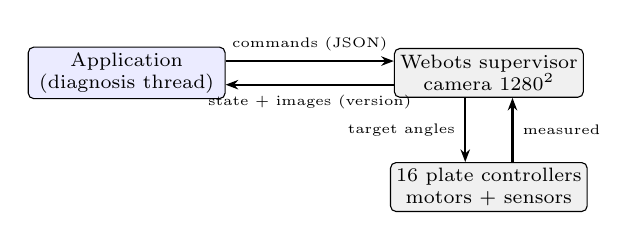
\begin{tikzpicture}[
			font=\scriptsize,
			box/.style={draw, rounded corners=2pt, align=center, minimum height=0.62cm, inner sep=2pt, fill=white},
			arr/.style={-{Stealth[length=1.6mm]}, thick}
			]
			\node[box, fill=blue!8, minimum width=2.5cm] (app) at (0,0) {Application\\(diagnosis thread)};
			\node[box, fill=gray!12, minimum width=2.4cm] (sup) at (4.6,0) {Webots supervisor\\camera $1280^2$};
			\node[box, fill=gray!12, minimum width=2.4cm] (pan) at (4.6,-1.45) {16 plate controllers\\motors + sensors};
			\draw[arr] ([yshift=1.5mm]app.east) -- node[above, font=\tiny]{commands (JSON)} ([yshift=1.5mm]sup.west);
			\draw[arr] ([yshift=-1.5mm]sup.west) -- node[below, font=\tiny]{state + images (version)} ([yshift=-1.5mm]app.west -| app.east);
			\draw[arr] ([xshift=-3mm]sup.south) -- node[left, font=\tiny]{target angles} ([xshift=-3mm]pan.north);
			\draw[arr] ([xshift=3mm]pan.north) -- node[right, font=\tiny]{measured} ([xshift=3mm]sup.south);
		\end{tikzpicture}
		\caption{Live testing loop. The application misaligns the simulated plates and compares each diagnosis with the angles measured in the simulation.}
		\label{fig:live}
	\end{figure}

	\begin{table}[!t]
		\centering
		\caption{Commands of the Live Testing Mode}
		\label{tab:live}
		\scriptsize
		\setlength{\tabcolsep}{2pt}
		\renewcommand{\arraystretch}{1.08}
		\begin{tabularx}{\columnwidth}{@{}P{1.5cm} Y@{}}
			\toprule
			Command & Effect\\
			\midrule
			Zero & All plates to $(0,0)$; the next stable image becomes the reference\\
			Random & $N$ random plates to random angles up to a given limit; the rest to zero\\
			Plate & One plate to a given $(\theta_1,\theta_2)$\\
			Scene & Camera pose and lights randomized as in the dataset, or restored\\
			\bottomrule
		\end{tabularx}
	\end{table}

	A diagnosis is only meaningful if the image was taken with the plates at rest in the configuration whose angles are reported. For this reason, every command increments a version number, and an image carries that version only when all the plates have reported being at their target for several consecutive steps; otherwise, it carries zero. The application analyzes automatically, exactly once per version, the first image whose version matches that of a stable state, and displays the measured angles as ground truth together with the error of each plate. In this way, each command produces one diagnosis that can be compared directly with the simulation, and changing the scene tests the robustness to the camera pose without moving the plates. The communication and the automatic analysis were verified against an emulated supervisor; a systematic evaluation in this mode is part of the future work.


	\section{Conclusions}

	A single overhead photograph with four fiducial markers is sufficient to estimate the 32 joint angles of a SOFIA module: rectification removes the effect of the camera pose, and the resulting top view allows both a training-free geometric estimator and learned regressors. With the simulation model of the unit and 10\,000 synthetic images whose misalignments follow the expected operation of the robot, a small CNN achieves a mean error of $0.20^\circ$, a maximum error of $3.3^\circ$, and a state accuracy of 96.8\,\%, and is the most accurate estimator in every range; the geometric method, limited by the short lever arm of the unit, remains a fallback when no GPU or training data are available, and the hybrid rule no longer provides an advantage. The estimators were integrated in a threaded diagnosis application that also connects to a live Webots simulation, which allows the complete chain, from misalignment to diagnosis, to be tested without the physical module. Future work includes a systematic evaluation in the live mode, the integration of the application as a diagnosis mode of the main SOFIA interface, and validating the CNN on photographs of the physical $4\times4$ module, fine-tuning it with real images to close the gap between simulation and reality.

	\balance

	\bibliographystyle{IEEEtran}
	\bibliography{bibliography}

\end{document}
